%%%%%%%%%%%%%%%%%%%%%%%%%%%%%%%%%%%%%%%%%%%%%%%%%%%%%%%%%%%%%%%%%%%%%%%%%%%%%
%%%
%%% File: utthesis2.doc, version 2.0jab, February 2002
%%%
%%% Based on: utthesis.doc, version 2.0, January 1995
%%% =============================================
%%% Copyright (c) 1995 by Dinesh Das.  All rights reserved.
%%% This file is free and can be modified or distributed as long as
%%% you meet the following conditions:
%%%
%%% (1) This copyright notice is kept intact on all modified copies.
%%% (2) If you modify this file, you MUST NOT use the original file name.
%%%
%%% This file contains a template that can be used with the package
%%% utthesis.sty and LaTeX2e to produce a thesis that meets the requirements
%%% of the Graduate School of The University of Texas at Austin.
%%%
%%% All of the commands defined by utthesis.sty have default values (see
%%% the file utthesis.sty for these values).  Thus, theoretically, you
%%% don't need to define values for any of them; you can run this file
%%% through LaTeX2e and produce an acceptable thesis, without any text.
%%% However, you probably want to set at least some of the macros (like
%%% \thesisauthor).  In that case, replace "..." with appropriate values,
%%% and uncomment the line (by removing the leading %'s).
%%%
%%%%%%%%%%%%%%%%%%%%%%%%%%%%%%%%%%%%%%%%%%%%%%%%%%%%%%%%%%%%%%%%%%%%%%%%%%%%%

\documentclass[a4paper, 12pt, oneside]{report}         %% LaTeX2e document.
\usepackage {tcdthesis}              %% Preamble.
\usepackage {graphicx}
\usepackage {placeins}

\mastersthesis                       %% Uncomment one of these; if you don't

%\thesisdraft                         %% Uncomment this if you want a draft
                                     %% version; this will print a timestamp
                                     %% on each page of your thesis.

\leftchapter                         %% Uncomment one of these if you want
%\centerchapter                      %% left-justified, centered or
% \rightchapter                      %% right-justified chapter headings.
                                     %% Chapter headings includes the
                                     %% Contents, Acknowledgments, Lists
                                     %% of Tables and Figures and the Vita.
                                     %% The default is \centerchapter.

% \singlespace                       %% Uncomment one of these if you want
\oneandhalfspace                     %% single-spacing, space-and-a-half
% \doublespace                       %% or double-spacing; the default is
                                     %% \oneandhalfspace, which is the
                                     %% minimum spacing accepted by the
                                     %% Graduate School.

\renewcommand{\thesisauthor}{Ben Lynch}                     %% Your official UT name.
\renewcommand{\thesismonth}{September}                      %% Your month of graduation.
\renewcommand{\thesisyear}{2017}                            %% Your year of graduation.
\renewcommand{\thesistitle}{Investigating the Energy Consumption of Member Discovery in Bluetooth Low Energy}
\renewcommand{\thesisauthorpreviousdegrees}{B.A.(Mod.)}     %% Your previous degrees, abbreviated; separate multiple degrees by commas.
\renewcommand{\thesissupervisor}{Jonathan Dukes}            %% Your thesis supervisor; use mixed-case and don't use any titles or degrees.

\renewcommand{\thesisauthoraddress}{ 11 Brookwood Heights, Artane, Dublin 5}

%%%%%%%%%%%%%%%%%%%%%%%%%%%%%%%%%%%%%%%%%%%%%%%%%%%%%%%%%%%%%%%%%%%%%%%%%%%%%%%%
%%% The following commands are all optional, but useful if your requirements
%%% are different from the default values in utthesis.sty.  To use them,
%%% simply uncomment (remove the leading %) the line(s).

\renewcommand{\thesisdegree}{Master in Computer Science}

\renewcommand{\thesisdegreeabbreviation}{MCS}

%%%%%%%%%%%%%%%%%%%%%%%%%%%%%%%%%%%%%%%%%%%%%%%%%%%%%%%%%%%%%%%%%%%%%%%%%%%%%%%%


\begin{document}                                  %% BEGIN THE DOCUMENT

\thesistitlepage                                  %% Generate the title page.

\thesisdeclarationpage				                    %% Generate the declaration page.

\thesispermissionpage				                      %% Generate the copyright permission page

\begin{thesisacknowledgments}
I would like to thank my supervisor Jonathan Dukes for suggesting such an interesting
project and assisting me throughout.

\end{thesisacknowledgments}


\begin{thesisabstract}
...ABSTRACT...
\end{thesisabstract}


\tableofcontents                                  %% Generate table of contents.
\listoftables                                     %% Uncomment this to generate list of tables.
\listoffigures                                    %% Uncomment this to generate list of figures.

%%
%% Include thesis chapters here...
%%
  \chapter{Introduction}

	\section{Introduction}
	Attendance tracking is commonly used in places such as universities, to determine
	student attendance in lectures, and in organisations, for taking employee attendance
	and for assembly scenarios such as in fire evacuation procedures.

	Attendance tracking has mainly been achieved by performing manual roll calls using
	pen and paper, but has had implementations using technologies such as barcodes,
	Radio-frequency identification (RFID), and Near field communication (NFC).
	In the case of barcodes and NFC, these technologies require users to manually
	scan themselves for their attendance to be taken. In the case of RFID, tag collision
	can occur when numerous tags in the same area respond at the same time. Although
	implementations exist using these technologies, they have limitations and are
	not always effortless for the user.

	Bluetooth Low Energy (BLE) is a version of Bluetooth which was designed specifically
	with the Internet of Things (IoT) in mind. It has ultra-low peak, average, and idle
	power consumption and operates in the industrial, scientific, and medical (ISM)
	radio band (2.400 - 2.4835 GHz). BLE has two modes of communication, broadcasting
	and connections, with broadcasting most commonly being used to discover devices in order
	to establish connections.

	Microcontrollers with BLE radios, such as Nordic Semiconductor's nRF51 series
	devices, are extremely small (6mm x 6mm x 1mm) and relatively cheap (from 2 euro).
	It is feasible to incorporate these microcontrollers into student or organisation
	ID cards. With the addition of energy efficient applications with a focus on radio
	duty cycling, a microcontroller should be able to run on a coin cell battery
	for the lifecycle of the ID card.

	High crowd density is one of the main characteristics of scenarios where
	attendance tracking is commonly used. With the use of multi-hop routing,
	this high crowd density can be exploited to reduce the required transmission
	range of devices, which in turn reduces the transmission power required.

	The combination of a low power routing protocol, such as the Ad-hoc On Demand
	Distance Vector routing protocol, with the exclusive use of BLE broadcasting results
	in an implementation with small packet sizes, low packet processing times, and
	removes the overhead of connection establishment, creating an ideal framework
	for efficient and long lasting attendance tracking applications.

	\section{Problem Area}
	As mentioned, the attendance tracking is focused in areas of high crowd densities.
	Devices in the location where attendance tracking is taking place will form wireless,
	mobile ad-hoc networks (MANET).

	Attendance tracking in MANETs is a form of network member discovery and so one of
	the most important requirements in the selection of an appropriate routing protocol
	is its performance in the discovery of new routes. Once a route is established,
	member presence knowledge will have been acquired and the route will only be used
	in the establishment of other routes.

	Energy efficiency will be one of the main requirements for an attendance tracking
	application, as it will have to last for the lifetime of the user's ID card. For
	the purpose of this research we consider that lifetime to be a year. The main
	mechanism to achieve this energy efficiency is radio duty cycling. That is, the
	radio of the device will remain in a low power mode for the majority of its life,
	only entering a higher power mode when attendance is being taken.

	\section{Motivation for this research}
	The Internet of Things (IoT) has recently been in the spotlight as one of the fastest
	growing information technology sectors. According to a report \cite{IHS_IOT} from
	the financial services company IHS Markit, the number of IoT devices is expected
	to rise by fifteen percent year-over-year to reach twenty billion in 2017.

	According to the IoT Developer Survey 2017 \cite{SURVEY_IOT}, Bluetooth Low Energy
	has seen a growth of twelve percent in its use as a connectivity protocol for IoT solutions
	since 2015. In addition to this, the majority of major android branded
	smartphones (Android OS 4.3 and above), iOS devices (model 4S and onwards),
	and Windows based smart phones are BLE enabled. The early adoption of BLE in Apple's
	iBeacon has also aided in the wider adoption of BLE technology.

	The explosion of the IoT and the growing adoption rate of BLE make it an exciting
	technology to work with. It is still a relatively new technology and further
	research into its capabilities and possible applications is still required.

	\section{Objectives}
	The goals of this dissertation are as follows:
	\begin{itemize}
		\item The design of an attendance tracking protocol based on an existing routing
		protocol suitable for member identification in an ad-hoc network.
		\item The implementation of a module encapsulating the functionality of the
		chosen routing protocol.
		\item The implementation of an application which makes use of the above module
		to track attendance.
		\item An analysis of the performance of the protocol in BLE.
	\end{itemize}

	\section{Dissertation Outline}
	This dissertation begins with a literature review in Chapter 2 which provides
	an understanding of radio duty cycling, an overview of appropriate routing
	protocols, and a review of their performance. Chapter 3 provides a description of the key aspects of BLE for the
	development of applications, a discussion of design decisions related to the implementation
	of a routing protocol for BLE, as well as a description of two protocols
	for attendance tracking. Chapter 4 discusses the implementation of these protocols
	and provides some security considerations with regards to the implementation.
	Chapter 5 provides an overview of the evaluation methodology, results from medium
	scale testing, and an analysis of these results. Finally, Chapter 6 summarises the
	contributions made by this dissertation, a general discussion on the outcome of this thesis, and areas
	for future work.

  \chapter{Background} \label{background}

    \section{Introduction}
    This chapter investigates some of the techniques currently used in radio duty cycling,
    a key component in low energy applications. Specifically, an overview of the X-MAC, Box-MAC-2,
    and ContikiMAC radio duty cycling protocols is provided along with the benefits
    associated with the techniques used.

    An overview of well known ad-hoc routing protocols is also provided with a focus
    on route discovery as a mechanism for attendance tracking, and packet size,
    as BLE advertisement packets are limited in size. A brief overview on research
    related to the performance of these protocols is then provided.

    \section{Radio duty cycling}
    Power consumption is extremely important for nodes that wish to achieve a long
    network lifetime. It is not possible to achieve this long life time if a radio transceiver
    is permanently powered on as even low-power transceivers consume too much power.
    By turning the radio transceiver off a node can conserve energy and achieve a
    long network lifetime, however when the transceiver is off, the node cannot
    send or receive messages. This is solved by keeping the radio off only in-between
    the reception and transmission of messages.

      \subsection{Low Power Listening}
    Low Power Listening (LPL) \cite{LPL} is a duty cycling technique in which receivers periodically
    turn on their radios to identify if there is activity in the radio medium. If
    activity is detected, the receiving node's radio is kept on for a longer period
    so that data can be exchanged. an illustration of LPL is provided in figure \ref{fig:lpl}.

    \FloatBarrier
    \begin{figure}[ht]
      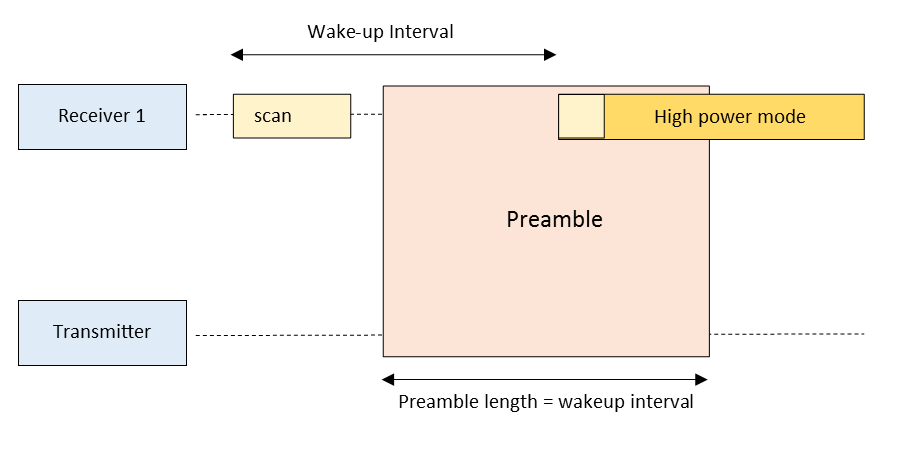
\includegraphics[width=\textwidth]{Images/chapter2/lpl.png}
      \caption{Low Power Listening}
      \label{fig:lpl}
    \end{figure}
    \FloatBarrier

    Transmitting nodes send a preamble stream which is at least as long as the
    receiving node's wake-up interval, ensuring that the receiver will have their
    radio on during the transmission of the preamble. When a receiving node detects
    a preamble stream, they respond with an acknowledgement, and the transmitting
    node terminates the preamble transmission.

    LPL was designed for single node wake-up. Broadcast mode is possible, however,
    this requires the transmission of maximum length preamble streams as the transmitting
    node does not know when all intended receivers have woken up, and single node
    wake-up is rendered impossible as any node detecting the preamble will keep
    their radio on afterwards.

      \subsection{Low Power Probing}
    Low Power Probing (LPP) \cite{LPP} is a duty cycling technique in which the roles from LPL
    are reversed. Instead of receivers scanning at wake-up intervals, they periodically
    broadcast a probe package. an illustration of LPP is provided in figure \ref{fig:lpp}.

    \FloatBarrier
    \begin{figure}[ht]
      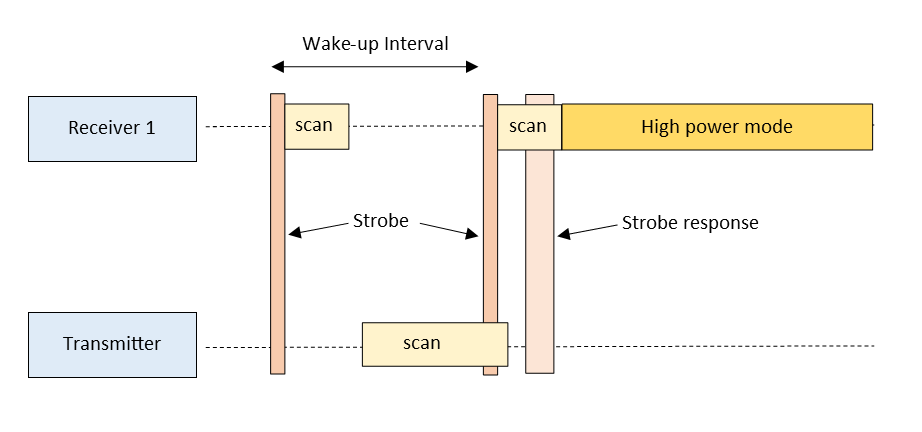
\includegraphics[width=\textwidth]{Images/chapter2/lpp.png}
      \caption{Low Power Probing}
      \label{fig:lpp}
    \end{figure}
    \FloatBarrier

    Transmitting nodes scan until a probe is detected, at
    which point they immediately transmit a probe response. The receiver scans for a short
    period after sending a probe, ensuring it will receive any probe responses
    intended for it. Upon receiving data, the receiver will enter a high power mode,
    keeping their radio on for a longer period.

      \subsection{X-MAC}
    X-MAC \cite{XMAC} is an LPL based radio duty cycling protocol. X-MAC implements
    a variation of LPL in which the transmitting node sends a series of short
    preamble packets which include the address of the target destination. Periodic gaps
    are used during the transmission of these shorter preambles. By including the
    destination address, receiving nodes are able to turn their radios off immediately
    if they are not the destination specified. The periodic gaps in the transmitting node's
    preamble stream are used by receiving nodes to send acknowledgements. This
    series of short preambles approximates the continuous preamble from standard
    LPL. The X-MAC protocol is illustrated in figure \ref{fig:xmac}.

    \FloatBarrier
    \begin{figure}[ht]
      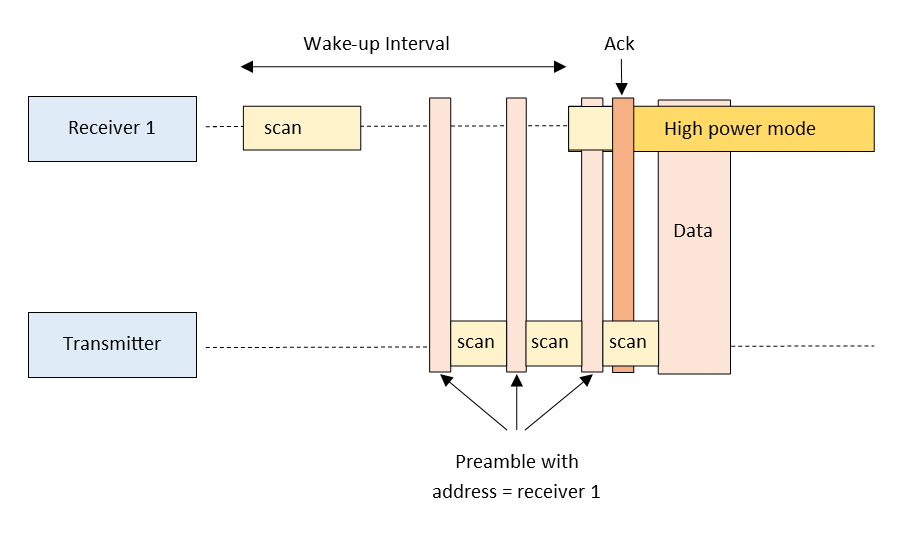
\includegraphics[width=\textwidth]{Images/chapter2/xmac.png}
      \caption{X-MAC}
      \label{fig:xmac}
    \end{figure}
    \FloatBarrier

    The inclusion of a destination address reduces the wake-up cost for nodes which
    preambles are not intended for, making single-node wake-up feasible using
    broadcasting.

      \subsection{BoX-MAC-2} \label{box_mac}
    BoX-MAC-2 \cite{BOX_MAC} is an adaptation of X-MAC in which a transmitting node
    includes the entire data packet within the preamble, instead of the destination
    address. This eliminates the need for a transmitting node to send further
    data after receiving an acknowledgement from a receiving node. The Box-MAC-2 protocol
    is illustrated in figure \ref{fig:boxmac2}.

    \FloatBarrier
    \begin{figure}[ht]
      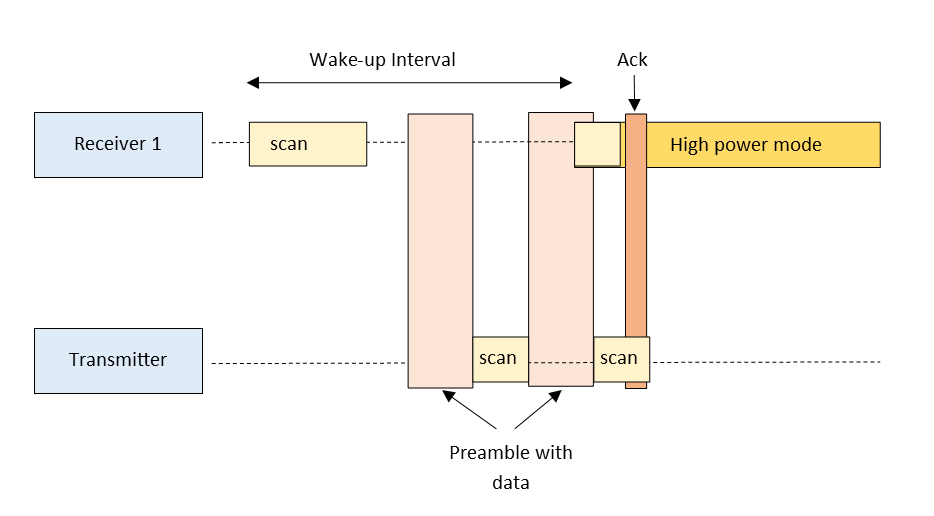
\includegraphics[width=\textwidth]{Images/chapter2/boxmac2.png}
      \caption{Box-MAC-2}
      \label{fig:boxmac2}
    \end{figure}
    \FloatBarrier

      \subsection{ContikiMAC}
    ContikiMAC \cite{ContikiMAC} is a radio duty cycling protocol that uses LPL and is based on
    X-MAC. It has two unique mechanisms to reduce energy consumption which can be
    seen in figure \ref{fig:contikimac}.

    The first mechanism is \textit{Fastsleep}. With this, nodes turn off their radios if one
    of three conditions are met:
    \begin{itemize}
      \item if a node detects radio activity longer than the largest packet length
      in the protocol.
      \item if detected radio activity is followed by a silence period which is
      longer than two successive transmission intervals.
      \item if valid radio activity is identified but no start of packet could be
      detected.
    \end{itemize}

    The second mechanism is \textit{Transmission Phase Lock}. With this, each node maintains
    the wake-up phases of their neighbours by noting the time at which it saw link
    layer acknowledgements from them during its wake-up phase. With this information
    a node can send information to its neighbour when it knows the neighbour will be awake.

    \FloatBarrier
    \begin{figure}[ht]
      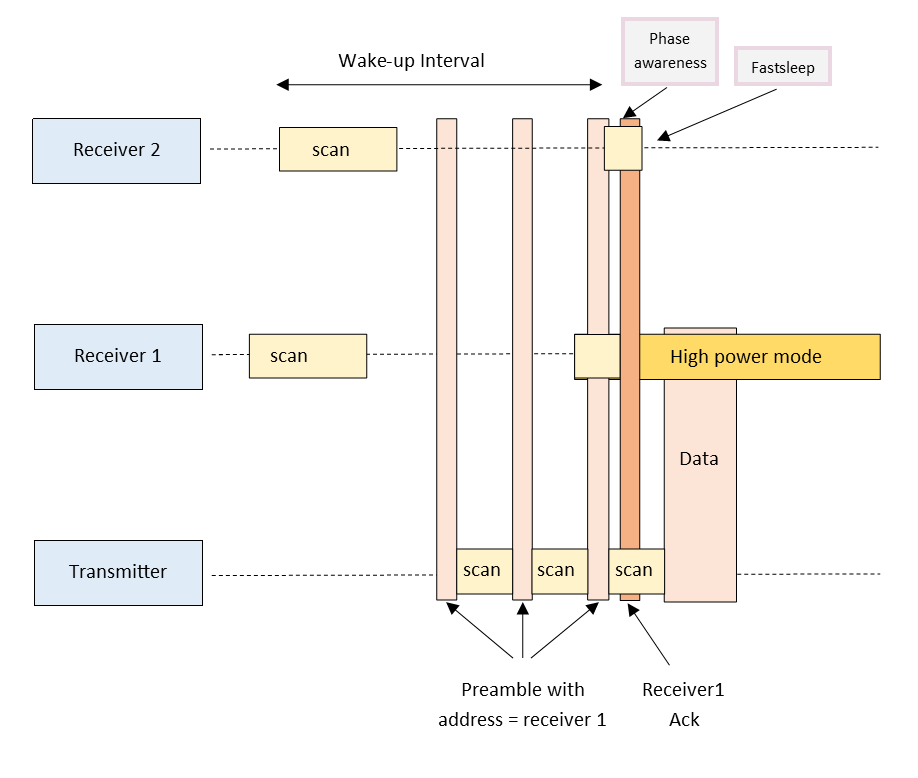
\includegraphics[width=\textwidth]{Images/chapter2/contikimac.png}
      \caption{ContikMAC}
      \label{fig:contikimac}
    \end{figure}
    \FloatBarrier

    According to the ContikiMAC radio duty cycling protocol report \cite{ContikiMAC},
    in which the protocol was evaluated in the Contiki simulation environment,
    it was found that the Fastsleep and Phase Lock mechanisms reduce network power
    consumption by between 10 and 80 percent, depending on the wakeup frequencies of
    devices.

    \section{Routing Protocols} \label{routing_protocols}
      \subsection{Ad-hoc On Demand Distance Vector routing}
        \subsubsection{Overview}
    Ad-hoc On Demand Distance Vector routing (AODV) \cite{RFC3561} is a reactive routing protocol
    designed for use in mobile ad-hoc networks. In AODV, topology information is only
    transmitted on demand. Only a single route is ever recorded between a source
    and destination, and is only maintained while active. An example of route discovery
    in AODV can be seen in figure \ref{fig:adov}.

    \FloatBarrier
    \begin{figure}[ht]
      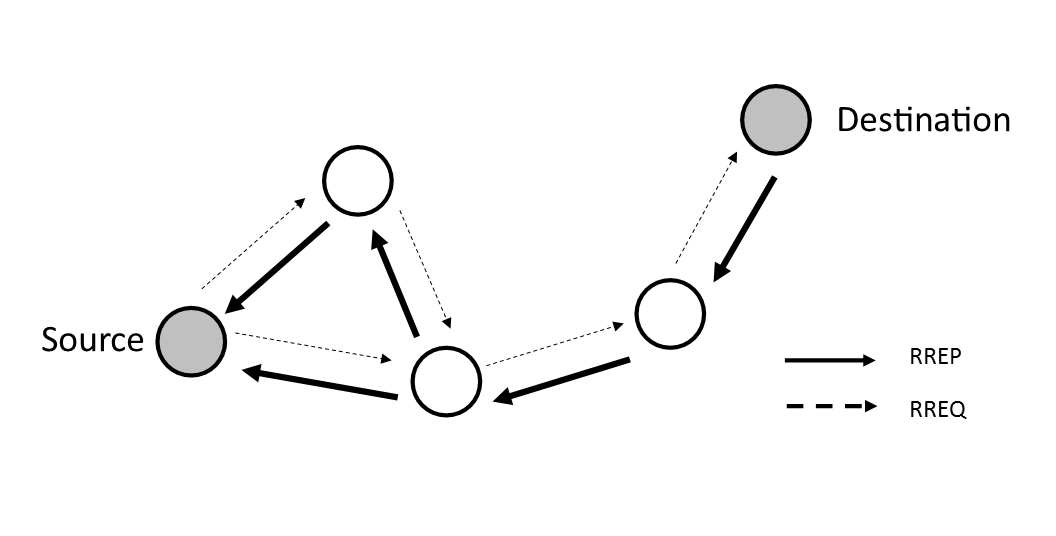
\includegraphics[width=\textwidth]{Images/chapter2/aodv.png}
      \caption{AODV route discovery}
      \label{fig:adov}
    \end{figure}
    \FloatBarrier

    The AODV protocol has built in sequencing numbers in each of its control
    packets which prevents routing loops being formed, a challenge faced by many
    routing algorithms. In addition to this, each node maintains its own routing
    table, keeping the routing process minimal if the host has the required
    route information in its own routing table. Entries in the routing table
    have a time to live and if not used will expire, limiting the memory overhead
    to routes that are being used, as opposed to all possible routes.

    When a node wishes to send traffic to a host and no route is known, a \textit{route
    request} (RREQ) message is broadcast. At each node the RREQ arrives at, the
    following processing takes place:
    \begin{itemize}
      \item The node creates or updates a route to the previous hop from which
      the RREQ was received.
      \item If a RREQ with the same source address and RREQ ID has been previously
      received within a certain time period, the RREQ is discarded.
      \item The node increments the Hop Count within the RREQ by one.
      \item The node creates or updates a reverse route to the source address of
      the RREQ. This is required in the event a RREP is received with the source
      of the RREQ as the destination.
      \item If the node is the destination of the RREQ, it discards the RREQ,
      generates a RREP, and sends the RREP to the next hop of the reverse route.
      \item If the node is not the destination but has a routing table entry
      for the destination, it can generate a  route reply (RREP) which it sends to the RREQ source.
      \item If the node is not the destination and does not have any routing information
      regarding the destination, it re-broadcasts the RREQ message.
    \end{itemize}

    At each node a RREP arrives at, the following processing takes place:
    \begin{itemize}
      \item The node creates or updates a route to the previous hop from which
      the RREP was received.
      \item The node increments the Hop Count within the RREP by one.
      \item The node creates or updates a route to the source of the RREP.
      \item The node sends the RREP to the next hop indicated in the routing
      table entry for the RREP's destination address.
    \end{itemize}

    In summary, a route is considered found when the RREQ message arrives at either the desired host,
    or to an intermediary node with a valid route entry for the destination.
    In either case, a RREP is sent back to the originator of
    the RREQ message. As the RREP message propagates back to the originator,
    each intermediary node creates a route to the destination (the source of the
    RREP).

    Route maintenance is performed using Hello messages which detect link breaks. Nodes periodically
    broadcast these Hello messages to their neighbours and in the event that a
    node fails to receive a Hello message within a certain period from its neighbour,
    a break is detected. In the event that a node detects an error in one of its known
    routes, it sends a route error (RERR) message to each of its neighbours.

        \subsubsection{Control Packets}
    Figures \ref{fig:adov_rreq} and \ref{fig:adov_rrep} show the format
    of AODV's two primary control packets, RREQs and RREPs.
    \FloatBarrier
    \begin{figure}[ht]
      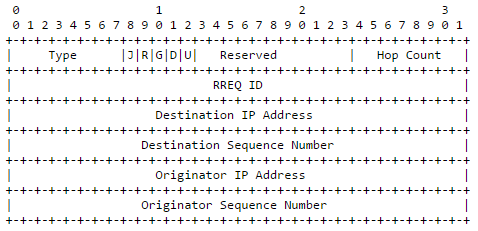
\includegraphics[scale=0.75]{Images/chapter2/aodv_rreq.png}
      \caption{AODV RREQ packet format}
      \label{fig:adov_rreq}
    \end{figure}
    \FloatBarrier

    \FloatBarrier
    \begin{figure}[ht]
      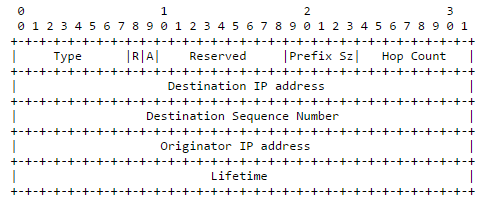
\includegraphics[scale=0.75]{Images/chapter2/aodv_rrep.png}
      \caption{AODV RREP packet format}
      \label{fig:adov_rrep}
    \end{figure}
    \FloatBarrier

    These are static sized packets with the RREQ packet having a total size of
    twenty-four bytes and the RREP packet having a total size of twenty bytes.

      \subsection{Dynamic Source Routing}
    Dynamic Source Routing (DSR) \cite{RFC4728} is a routing protocol designed
    for multi-hop wireless ad-hoc networks of mobile devices. DSR is based on a type
    of routing called \textit{source routing}. In source routing, the sender of a packet
    determines the complete route in which a packet is to be forwarded through.

    Each node in the network maintains a route cache in which it caches source routes
    which it has learned of. When sending a packet, the node first checks for a valid
    route to the destination in its route cache. If a route is found, it is used
    to transmit the packet. If no route is found, the node can discover the route
    using DSRs route discovery protocol.

    Nodes initiating route discovery broadcast a route request (RREQ) packet identifying
    both the source of the RREQ and the target node. Each RREQ message contains
    a \textit{route record}, which is the accumulated sequence of hops taken by
    the RREQ packet as it propagates through the network. Upon reaching the target
    destination, a \textit{route response} (RREP) packet is generated containing the
    route by which the RREQ arrived through. This RREP is then returned via a route
    specified in the nodes route cache if one exists, or by reversing the route
    contained in the RREQ.

    Route maintenance is performed by every node in a route. If a node exceeds
    it's maximum number of retransmissions for a packet it is forwarding without
    receiving a response, it must send a \textit{route error} message to the original
    sender of the packet.

      \subsubsection{Control Packets}
    Figure \ref{fig:dsr_rreq} and figure \ref{fig:dsr_rreq} show the format
    of DSR's two primary control packets, RREQs and RREPs.

    \FloatBarrier
    \begin{figure}[ht]
      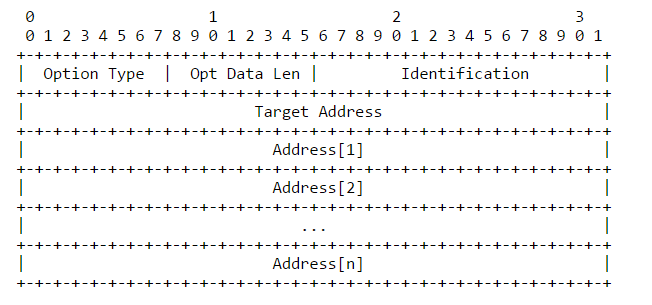
\includegraphics[scale=0.75]{Images/chapter2/dsr_rreq.png}
      \caption{DSR RREQ packet format}
      \label{fig:dsr_rreq}
    \end{figure}
    \FloatBarrier

    \FloatBarrier
    \begin{figure}[ht]
      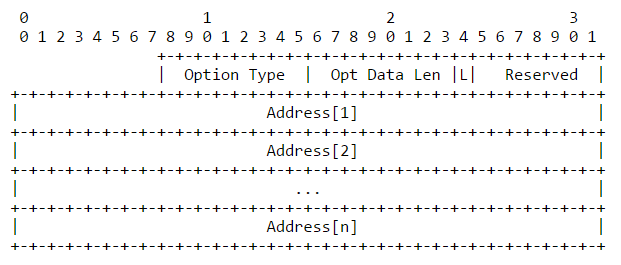
\includegraphics[scale=0.75]{Images/chapter2/dsr_rrep.png}
      \caption{DSR RREP packet format}
      \label{fig:dsr_rreq}
    \end{figure}
    \FloatBarrier

    These are dynamic sized packets, with the RREQ having an eight byte header
    with n possible addresses each of which are four bytes. This list grows as the
    RREQ propagates through the network. The RREP packet has a four byte header
    with n possible addresses, again, each of which are four bytes each. This list
    identifies the route the packet should take.

      \subsection{Optimised Link State Routing}
    Optimised Link State Routing (OLSR) \cite{RFC3626} is proactive IP routing protocol
    optimized for mobile ad hoc networks. Proactive protocols are those in which
    routing information for all nodes in the network is discovered and maintained
    before the transmission of packets. It is an optimisation of a pure link state
    protocol for mobile ad-hoc networks. In pure link state protocols, all adjacent
    network links are flooded through the entire network. In
    DSDV, only a subset of these links are declared. This subset is known as the
    \textit{multipoint relay selectors}. In addition to this, flooding of control
    traffic is minimised as nodes only use the selected nodes, called \textit{multipoint
    relays} (MPR) to transmit traffic to the rest of the network.

    HELLO messages are used for neighbour sensing. They are broadcast to all
    nodes within one-hop but are not relayed to further nodes. They contain
    information relating to neighbours and their link status. This allows
    a node to learn about nodes up to two hops away.

    Topology Control (TC) messages are periodically sent throughout the network
    using MPRs. These messages contain a list of neighbours who have selected
    the transmitting node as an MPR. The information in these nodes are used by
    receiving nodes to build topology tables, which identify the MPRs used by
    each node in the network, and are used to calculate routing tables.

        \subsubsection{Control Packets}
    Figure \ref{fig:olsr_hello} and figure \ref{fig:olsr_tc} show the format
    for OSLR's two primary control packets, HELLO and TC.
    \FloatBarrier
    \begin{figure}[ht]
      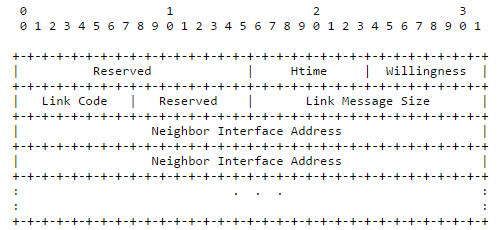
\includegraphics[scale=0.75]{Images/chapter2/olsr_hello.png}
      \caption{OLSR HELLO packet format}
      \label{fig:olsr_hello}
    \end{figure}
    \FloatBarrier

    \FloatBarrier
    \begin{figure}[ht]
      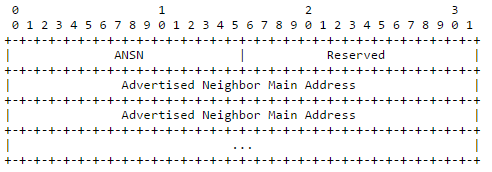
\includegraphics[scale=0.75]{Images/chapter2/olsr_tc.png}
      \caption{OLSR TC packet format}
      \label{fig:olsr_tc}
    \end{figure}
    \FloatBarrier

    The HELLO packet contains eight bytes of header information and a list of n neighbour
    addresses which are four bytes each. The TC packet contains a four byte header and
    a list of n node addresses which are again four bytes each.

      \subsection{Destination Sequenced Distance Vector Routing}
    Destination Sequenced Distance Vector Routing (DSDV) \cite{DSDV} is a table driven
    routing protocol designed for ad hoc mobile networks. DSDV uses the Bellman-Ford algorithm with a hop count
    metric to calculate paths. The Bellman-Ford algorithm \cite{bellman} computes the shortest
    path from a source vertex to all other vertices in a weighted graph.
    DSDV is a proactive protocol, meaning the routing information for all nodes
    in the network is maintained in the routing table and routes are added
    and updated by nodes exchanging table information at regular intervals and
    through triggers mechanisms employed by the protocol.

    Each node in the network maintains its own sequence number which is independently
    chosen. Each time a periodic update is made, a node increments its sequence
    number by two. Every update sent by a node includes their sequence number
    to eliminate routing loops.

      \subsubsection{Control Packets}
    There are two defined packets in DSDV for advertising routing table information.

    The first type of packet is the \textit{full dump}. Full dumps carry all
    available routing information from a node and are intended for infrequent
    use. Full dump messages will most likely require multiple network protocol data
    units (NPDU).

    The second type of packet is the \textit{incremental}. Incremental packets
    contain routing information which has changed since the last full dump.
    Incremental messages are intended to fit within a single NPDU.

      \subsection{IPv6 Routing Protocol for Low-Power and Lossy Networks}
        \subsubsection{Overview}
    The Routing Protocol for Low-Power and Lossy Networks (RPL) \cite{RFC6550} is
    a distance vector IPv6 routing protocol designed for wireless ad-hoc
    sensor networks. The protocol specifies how to build
    a \textit{Destination Oriented Directed Acyclic Graph} (DODAG) using an objective
    function and a set of metrics and constraints. The objective function operates
    on this set of metrics and constraints. An example of an DODAG objective is
    to "Find the path with the lowest hop count(metric) while avoiding non-encrypted
    links (constraint)". An \textit{RPLInstance} is comprised of one or more DODAGs
    and multiple RPLInstances can be active in the network at a time, with nodes
    having multiple objective functions active at once.

    The graph building process begins at a root node. The root broadcasts information
    about the DODAG formation using DODAG Information Objects (DIO) packets. These
    packets carry relevant network information that allows nodes to discover the
    new RPLInstance, learn its configuration parameters, and to select a set of
    parent nodes. Nodes receiving DIOs decide whether to join the DODAG according
    to their objective function. Nodes joining the DODAG compute their rank within
    the DODAG, which is an indication of their co-ordinates within the graph hierarchy,
    and re-broadcasts the DIO message to their neighbours. The transmission of DIO packets
    build routes in the downwards direction from the root to leaf nodes. Nodes in
    the network can broadcast DODAG Information Solicitation (DIS) messages
    to solicit a DIO from surrounding RPL nodes.

    Point-to-point communications is achieved by sending packets 'up' the graph
    to a common ancestor, at which point the packet is forwarded 'down' to the
    desired destination.

        \subsubsection{Control Packets}
    Figure \ref{fig:rpl_pkt} illustrates the general format of RPL control packets.
    These packets have a four byte header and a base which contains DIS and DIO
    packets.

    \FloatBarrier
    \begin{figure}[ht]
      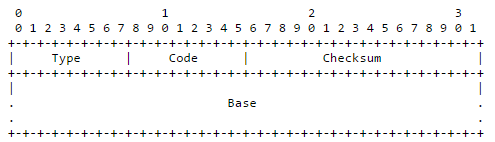
\includegraphics[scale=0.75]{Images/chapter2/rpl_pkt.png}
      \caption{RPL control packet format}
      \label{fig:rpl_pkt}
    \end{figure}
    \FloatBarrier

    DIS packets have a length of four bytes and can carry up to three
    IPV6 packet options which make up one byte.

    DIO packets are seven bytes long, including a 128 bit DODAGID, which is the
    IPv6 address belonging to the DODAG root.

    \section{Protocol Performance} \label{performance}
    This section provides an overview of some of the research conducted comparing
    the protocols found in section \ref{routing_protocols}.

    A performance comparison was performed between AODV and DSR in \cite{AODV_vs_DSR}.
    The comparison was performed using a simulation based on the NS-2 network simulator
    and focuses on low mobility networks. The performance metrics measured include:
    Packet Delivery Ratio (PDR) and End to end delay. The authors observed that
    AODV and DSR have very similar PDRs in static networks, but AODV has improved
    PDR with increased node movement. With respect to end to end delay, they observed
    that DSR marginally outperformed AODV in their simulations. Overall, they concluded
    that AODV is preferred to DSR due to its more efficient use of bandwidth.

    A performance comparison was performed between AODV and DSDV in \cite{AODV_vs_DSDV}.
    The comparison was performed using a simulator called MobiREAL which is also based
    on the NS2 network simulator. The performance metrics measured include:
    Network throughput and End to end delay. The authors observed that
    AODV had a PDR of seventy to ninety percent, while DSDV had a PDR of fifty to seventy-five percent. They observed
    high end to end delay initially in AODV that reduces with time, and the inverse in
    DSDV, with a low end to end delay in the beginning that gradually increases. They
    concluded that the performance of AODV was better than DSDV for real time applications.

    A performance comparison was performed between RPL and a lightweight version of
    AODV called LOADng in \cite{RPL_vs_AODV}. The simulated network is a static
    network which reflects the Home Automation \cite{roll_home} scenario. The comparison was performed using
    the Cooja simulator on the Contiki OS and uses the ContikiRPL implementation
    and a basic implementation of LOADng. The performance metrics measured include:
    End to end delay, Average hop distance, and Routing overhead. The authors
    observed that RPL provides shorter routes and a smaller spanning tree depth
    compared to LOADng in dense network topologies. They observed that the routing
    overhead of RPL largely depends on the choice of network parameters chosen but
    has less memory requirements than LOADng. They concluded that RPL performed
    better than LOADng but has a much higher implementation complexity. It is also
    worth noting that the LOADng implementation was unoptimised. If it was optimised
    it may have had better performance.

    A performance comparison was performed between DSDV, AODV, and DSR in
    \cite{DSDV_vs_AODV_vs_DSR}. The comparison was performed using the NS-2.34
    simulation tool. The performance metrics measured include: PDR, Network throughput,
    End to end delay, and Routing overhead. The authors observed that DSDV has a
    higher routing load and lower throughput compared to both AODV and DSR. AODV
    and DSR have extremely similar PDRs, end to end delays, and throughput in scenarios
    of low and high mobility, but AODV has a lower routing load in all tested scenarios.

    A performance comparison was performed between OLSR, AODV, and DSDV in
    \cite{OLSR_vs_AODV_vs_DSDV}. The comparison was performed with an NS-2 simulation
    with the simulated topologies being based on tactical networks for ships and
    sensor-based network nodes. The performance metrics used include: PDR, End to
    end delay, Routing overhead, and Normalised routing load. The authors observed
    that in scenarios of mobility, AODV outperforms both of the other protocols,
    with OLSR being a vast improvement over DSDV. In the scenario of a static
    sensor network OLSR outperformed AODV in all cases, with AODV performing
    poorly with high node density but still outperforming DSDV.

    From the above papers, AODV either outperforms or performs similarly to DSR
    regardless of network density or node mobility. AODV is superior to DSDV
    with respect to PDR, Routing Load, and Network throughput. It has worse
    end to end delay initially, but its end to end delay gradually improves, surpassing
    DSDV. AODV outperforms OLSR in all metrics in networks with node mobility, but
    the reverse is true in static networks. An unoptimised implementation of AODV is
    outperformed by RPL in all metrics within the Home Automation environment,
    a fully static sensor network. Although the above research does not focus on
    route discovery, it shows AODV as the most suitable protocol for networks with
    mobility and that it still performs well in static networks.

    \section{Summary}
    There are two primary methods of radio duty cycling, Low Power Listening and
    Low Power Probing. In LPL, duty cycling nodes scan for preamble streams at
    wake-up intervals. In LPP, duty cycling nodes advertise strobe
    packets at wake-up intervals followed by a short period of scanning. The X-MAC
    and Box-MAC-2 protocols have improved preamble usage, and ContikiMAC implements
    Fast Sleep and Transmission Phase Lock techniques to further improve the
    effectiveness of LPL radio duty cycling.

    There are many suitable routing protocols for low power ad-hoc networks.
    AODV is a reactive routing protocol that establishes routes on demand, uses the
    routing table at each intermediate device to establish routes, and has static
    sized packets. DSR is another reactive routing protocol but uses source
    routing in which the route is known before transmitting and so has dynamic
    sized packets. OLSR is a proactive protocol, meaning every node maintains
    a routing table representing the entire topology of the network. It is an
    optimisation of a pure link state protocol which uses Multipoint Relays to
    reduce the flooding of table information throughout the network. DSDV is another
    proactive protocol in which routing table information is periodically shared
    between neighbouring nodes and a Bellman-Ford algorithm is used to calculate
    paths. Finally, RPL is a protocol which specifies how to build a Destination
    Oriented Directed Acyclic Graph for sensor networks. Nodes in the network represent vertices
    and maintain information about their parents so that a path exists between
    any node and the root node.

    There have been some performance comparisons made between some of the
    protocols investigated in this chapter, all of which have been made using
    NS-2 or Cooja simulations. The main metrics measured are the Packet Delivery
    Ratio, End to end delay, and Routing overhead. AODV and DSR appear to have
    similar performance in static and mobile networks with DSR having a worse
    routing overhead. In the one experiment featuring RPL, it appears to outperform
    a light weight, unoptimised version of AODV, but has a much higher implementation
    complexity. In the one experiment featuring OLSR, it appears to have
    better overall performance than AODV in static topologies. DSDV appears to have
    the poorest performance out of all the routing protocols.

  \chapter{Methodology}

    \section{Introduction}

    \section{Protocol Assessment}
    Research - simulation

    \section{Custom Simulation}
      \subsection{Existing Simulators}
      \subsection{Custom Simulator Discussion}

    \section{Analysis of BLE Data Packets}

    \section{Summary}

  \chapter{Implementation}

    \section{Introduction}

    \section{nrf51}
      \subsection{nrf51 DK}
      \subsection{nrf5 SDK}
      \subsection{Nordic Python API}

    \section{Summary}

  \chapter{Results and Analysis}

    \section{Introduction}
    This chapter provides an overview of the methodology used in the evaluation
    of the implementation of the Roll Call \footnote{a short video demonstration of the Roll
    Call implementation is available at \cite{rc_demo}} and Route-to-Zero protocols. In addition to this, the
    results from a medium scale evaluation are shown and
    discussed.

    \section{Evaluation Methodology}
    The network topology used for the evaluation is a three by four grid with
    a root and nine user nodes as illustrated in figure \ref{fig:test_topology}. With this
    topology, the implementation can be tested with a hop count of three. A single hop
    is the maximum distance a node can broadcast data. From experiments with
    the nRF51 we discovered a hop distance of 4.32m when using a transmission
    power of -30 dBm (minimum transmission power of the nRF51).

    For this experiment the root node sends the RREQs alphabetically, beginning with
    node A and ending with node I.

    \FloatBarrier
    \begin{figure}[ht]
      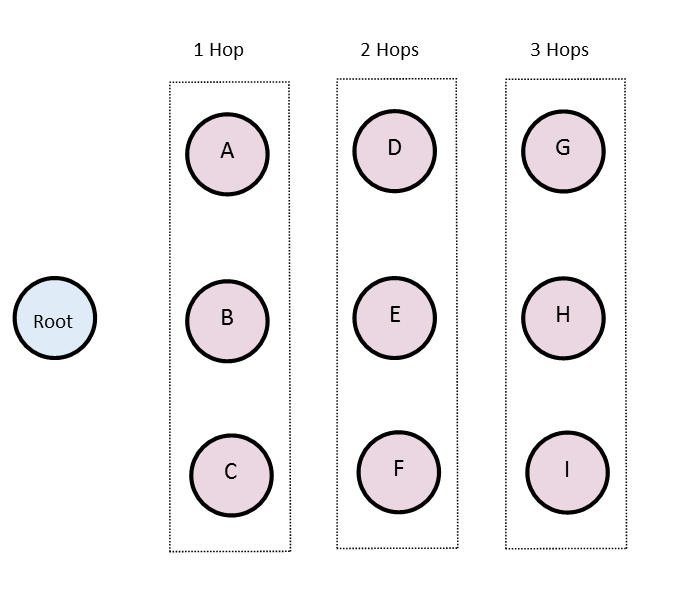
\includegraphics[scale=0.75]{Images/chapter5/setup.png}
      \caption{Evaluation network topology}
      \label{fig:test_topology}
    \end{figure}
    \FloatBarrier

    The metrics measured include:
    \begin{itemize}
      \item Node discovery rate.
            This is the rate at which nodes are discovered, measured from the
            beginning of the protocol until the final node has been identified.
            For the purpose of this experiment, the Route-to-Zero implementation
            knew the total number of nodes in the network.
      \item Total packets sent/processed per node.
            This is the total number of RREQ and RREP packets that are sent
            and processed by each node. Repeat packets are not processed.
      \item Average packets sent/processed per hop.
            This is the average number of packets sent and processed for each hop
            away from the root that a node is. Nodes A, B, and C are one hop away, nodes
            D, E, and F are two hops away, and nodes G, H, and I are three hops away.
    \end{itemize}

    These metrics were recorded using a statistics packet. This packet is sent
    to the root node in the same manner as a RREP packet. This packet contains
    the number of RREQs and RREPS that were received, sent, and processed by
    the node (repeat packets are not counted towards processed packet count).
    For the purpose of this experiment, all statistic packets were sent twenty
    seconds after the receipt of the first RREQ.

    \section{Medium Scale Evaluation Results}

    \subsection{Evaluation Settings}
    The BLE settings used in this experiment are as follows:
    \begin{itemize}
      \item Advertisement Interval: 100ms
      \item Advertisement Period: 500ms
      \item Scan Interval: 50ms
      \item Scan Window: 20ms
    \end{itemize}

    \subsection{Node discovery rate}
    The graph in figure \ref{fig:dsc_rate} shows the number of nodes that were
    discovered with respect to time.

    \FloatBarrier
    \begin{figure}[ht]
      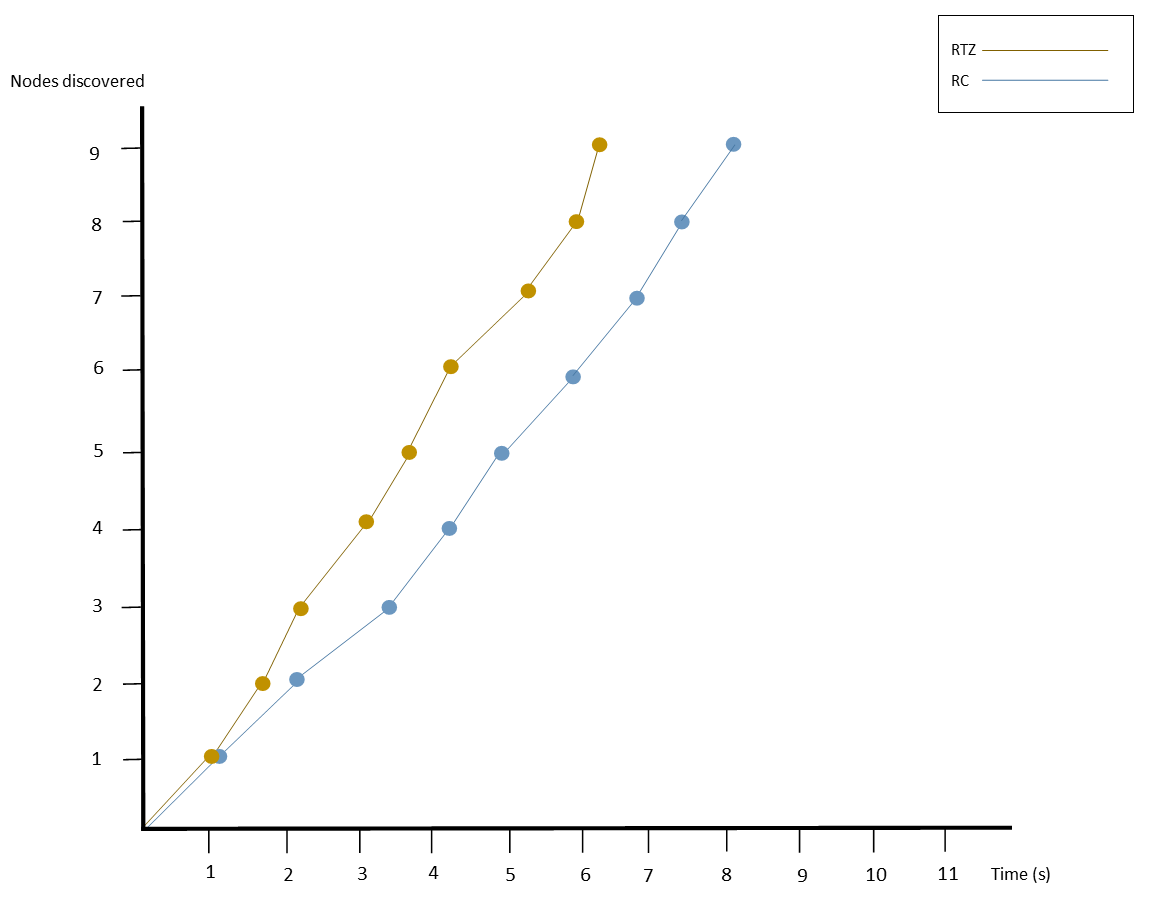
\includegraphics[width=\textwidth]{Images/chapter5/dsc_rate.png}
      \caption{Number of nodes discovered vs time}
      \label{fig:dsc_rate}
    \end{figure}
    \FloatBarrier

    Roll Call (RC) has a discovery rate of 1.06 nodes per second while Rout-to-Zero (RTZ)
    has a discovery rate of 1.34 nodes per second. The reason why RTZ has an improved
    discovery rate is that only a single RREQ is flooded through the network initially,
    meaning that nodes in the first hop can each send their own RREP after forwarding
    the RREQ, and as the wake-up RREQ arrives at subsequent hops, these nodes will
    have already performed a large chunk of the RREQ forwarding from other nodes
    and will we able to send their RREPs sooner than those in RC. In RC, the last
    RREQ from the root is only sent after 4.5 seconds (500ms per RREQ and 9 nodes),
    so when a RREQ arrives at its destination, the node will have its buffer filled
    with other messages to forward and so won't be able to respond with its own
    RREP as quickly. One important thing to note in this scenario is that when
    all nodes are discovered in RC no more packets will be broadcast within the network,
    whereas in RTZ, there may be RREP messages from the root still propagating
    through the network.

    \subsection{Packets per node}
    The graph in figure \ref{fig:pkts_node} shows the number of packets sent
    and processed at each node in the network.

    \FloatBarrier
    \begin{figure}[ht]
      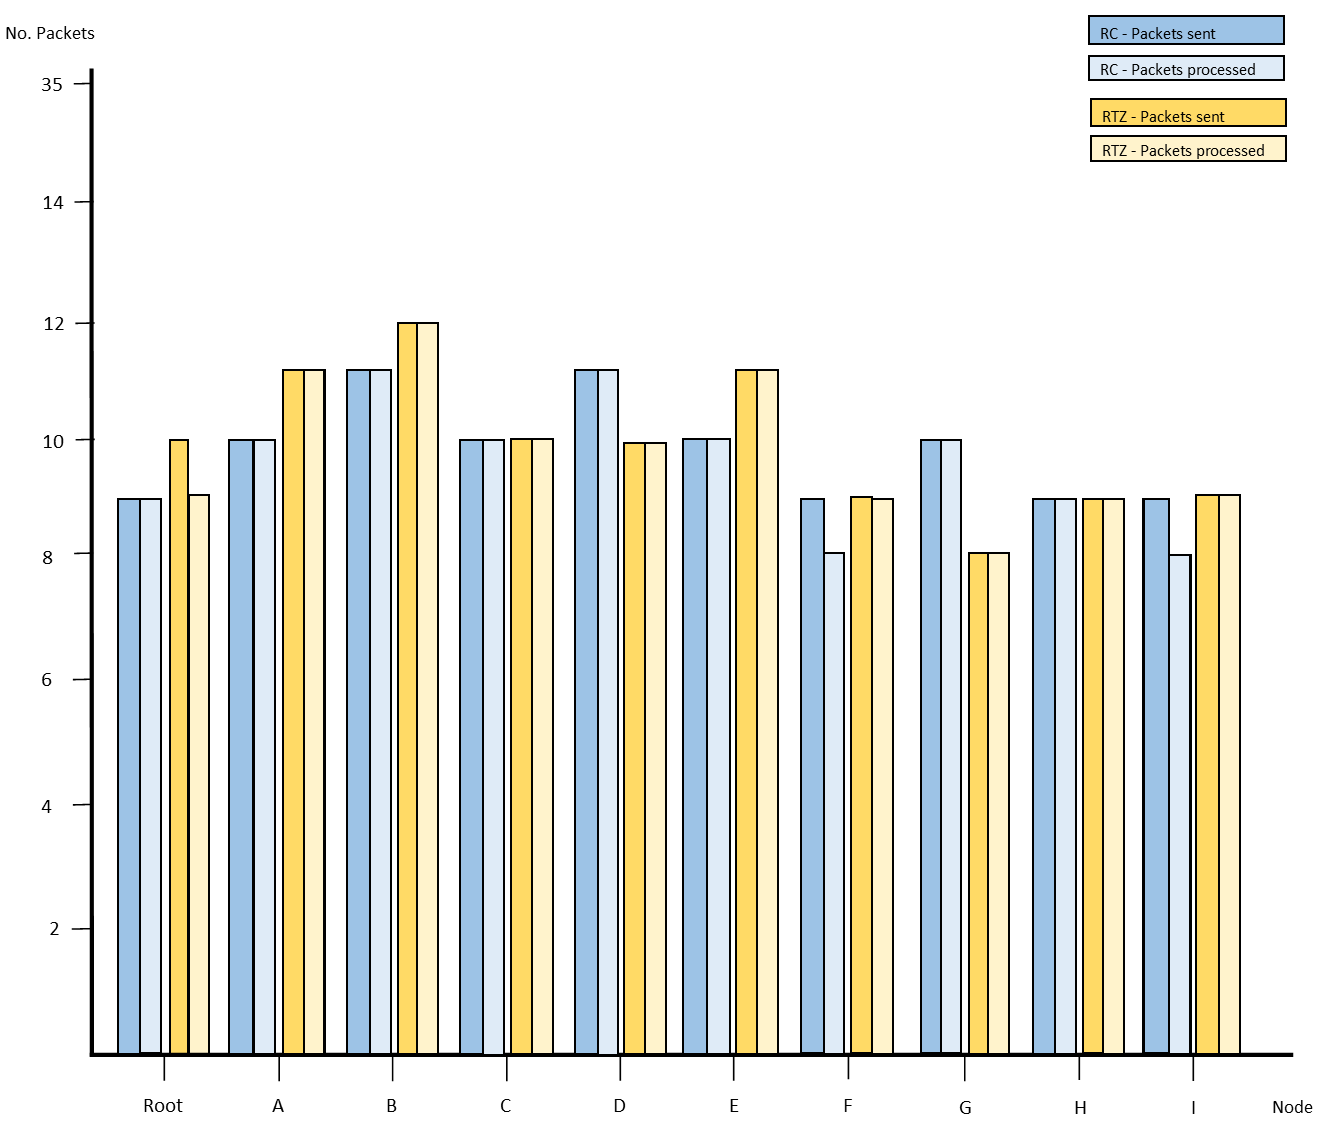
\includegraphics[width=\textwidth]{Images/chapter5/pkts_node.png}
      \caption{Total packets sent/received per node}
      \label{fig:pkts_node}
    \end{figure}
    \FloatBarrier

    The number of packets sent and processed at each node is very similar in both
    protocols and the number of sent packets is largely the same as the number of
    processed packets at each node.
    The reason for this is that if a RREQ is processed, it is either forwarded or a
    RREP is returned. If a RREP is processed, it will be forwarded as RREPs are
    only processed by nodes in the RREP route.

    The network will be flooded with
    repeat packets and broadcasted RREPs due to the nature of BLE advertising, but these packets will not
    have much impact on nodes as they are instantly discarded if repeated or not
    relevant.

    \subsection{Packets per hop}
    The graph in figure \ref{fig:pkts_hop} shows the average number of packets sent
    and received for nodes at different hop counts from the root.

    \FloatBarrier
    \begin{figure}[ht]
      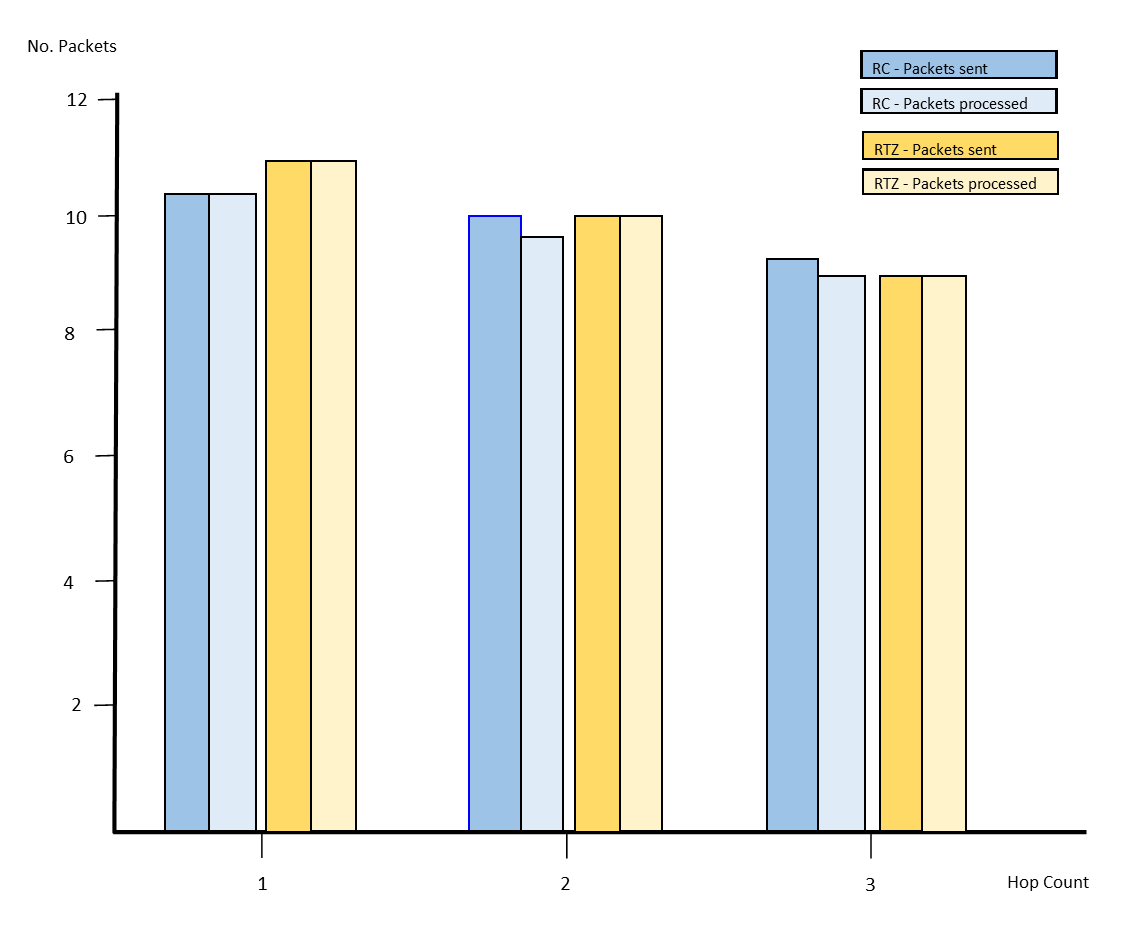
\includegraphics[width=\textwidth]{Images/chapter5/pkts_hop.png}
      \caption{Average packets sent/received vs hops from root}
      \label{fig:pkts_hop}
    \end{figure}
    \FloatBarrier

    The number of packets sent and received increases marginally the closer a node is to
    the root node. The reason for this is that nodes three hops away will not generally
    have any RREPs broadcast to them, so any that are scanned will likely be discarded and
    as a result, throughout the lifetime of the protocol the node will not have to forward any
    RREP packets. With an increased number of hops, and devices further apart, I
    expect this would result in more noticeable differences between hops.

    A difference in packet processing implies that nodes closer to the root consume more power than farther
    nodes as they are advertising for longer periods (if a node has no packets
    in its buffer advertising is turned off). This would only come into effect
    in networks with many more nodes than are present in this network. Nodes 1 hop from the root
    only advertise for \textasciitilde1s longer than those that are 3 hops away.

  \chapter{Conclusion}

  \section{Overview}
  In this thesis I have provided the design for two protocols that make use
  of AODV's route discovery mechanism to perform attendance tracking. The first
  protocol \textit{Roll Call}, is designed for lecture theatre-like scenarios in
  which the attendance of a pre-determined list of users is being taken. The
  second protocol \textit{Route to zero}, is designed for scenarios in which
  the attendance of a group of possibly unknown users is being taken.

  An AODV module with route discovery functionality was implemented for use in
  Bluetooth Low Energy. In addition to this, the Roll Call and Route-to-Zero protocols were implemented
  using the AODV module and tested in a small to medium scale network of nRF51
  devices. The results of the evaluation show the protocol working with three
  hops in the network, but further fine tuning of the BLE setting is required
  to improve the performance of the protocol.

  \section{Discussion}
  The two designs were capable of performing node discovery, but it is difficult
  to say how successful they were without any other references. Based on the recorded
  data, it would take the RTZ protocol 90 seconds to take the attendance in a lecture
  theatre of 120 students. This would be further increased in networks with mobility
  and in areas with high interference - an aspect of networks untested in this thesis.

  The AODV discovery mechanism was suitable for the task but in both designs, the amount
  of RREQ packets flooded through the system was quite high.
  It is possible that the metrics measured could be further improved by reducing
  the advertisement period and increasing the scanning interval, allowing for
  packets to be flooded through the network at a faster pace. It would also be necessary
  to experiment in larger networks - either with physical devices, or through
  simulation.

  Overall, AODV seems to have been a good choice. It outperformed the other
  investigated protocols in mobile networks, which could be desirable in attendance
  tracking applications, but was not tested in this thesis. For an approach
  focused on purely static networks, RPL or OLSR, would likely be better choices,
  but have a higher implementation complexity and their performance in BLE is
  difficult to predict.

  \section{Future Work}
  \subsection{Improvements to AODV}
  There are a number of improvements that could be made to the AODV module, namely
  the implementation of route maintenance. This would allow for attendance tracking
  in scenarios of high mobility and would be necessary in larger networks were there
  is a much higher chance of route failure.

  \subsection{Simulation}
  The testing of the designs outlined in this thesis was only performed in a small
  ten node network. It is difficult to test in larger physical networks as the devices
  have to be acquired, programmed, and space has to be located. With a minimum range
  of 4.32m, a very large space would be required to test networks with hop counts
  in the double digits and higher. One solution to this which is commonly used, is
  a simulation environment that replicates these larger networks which provides the
  advantage of not requiring physical devices or space.

  One issue with this is that there are few BLE simulation tools. There is a
  BLE simulator \cite{ble_simulator} implemented in the OMNeT++ simulator \cite{omnet}
  but there are no instructions, no updates, and it has quite poor code quality as
  it was initially intended to quickly check some of the author's ideas. As a
  result of this, in the early stages of this thesis, I decided to implement
  a higher level BLE simulator, which accurately simulated BLE channels in the
  physical layer, and advertising and scanning. The implementation was written
  in Java and drew from the OMNeT++ simulator. Unfortunately, there wasn't sufficient
  time to implement this as well as implementing the designs on physical hardware
  and so simulation development was halted to prioritise the physical implementation.

  \subsection{Implementation of other protocols}
  It would be interesting to implement some of the other protocols discussed in
  chapter \ref{background}, especially RPL. RPL outperformed AODV in
  section \ref{performance} so it would be interesting to see its performance
  when used for attendance tracking. The adaptation of RPL for
  BLE would be difficult as it has a very high implementation complexity but perhaps
  performance gains would outweigh this complexity.



\addcontentsline {toc}{chapter}{Appendices}       %% Force Appendices to appear in contents
\begin{appendix}
 \chapter*{Appendix}

...

\end{appendix}


%\addcontentsline {toc}{chapter}{Bibliography}     %% Force Bibliography to appear in contents

%\begin{thebibliography}[ieeetr]                 %% Start your bibliography here; you can
\bibliographystyle{ieeetr}
\bibliography{refs}                               %% also use the \bibliography command
%\end{thebibliography}                             %% to generate your bibliography.


\end{document}                                    %% END THE DOCUMENT
